\documentclass{beamer}
\usepackage{amsmath}
\usepackage{bbm}
\usepackage{stmaryrd}
\usepackage{ebproof}
\usepackage{tikz-cd}
\usepackage{array}

\newcommand{\kw}[1]{\ensuremath{ \mathrm{#1} }}
\newcommand{\bdot}{\boldsymbol{\cdot}}
\newcommand{\htr}[3]{{ {#1} \mathbbm{\{} {#2} \mathbbm{\}} {#3} }}
\setlength{\parskip}{1em}

\AtBeginSection[]
{
    \begin{frame}
        \frametitle{Table of Contents}
        \tableofcontents[currentsection]
    \end{frame}
}

\title{Refinement-Based Game Semantics for
  Certified Abstraction Layers}
\author{J\'er\'emie Koenig \and Zhong Shao}

\begin{document}

\begin{frame}
\titlepage
\end{frame}

\section{Introduction} %{{{

\begin{frame}{DeepSpec} %{{{
  Certified software this past decade:
  \begin{itemize}
    \item C compiler (CompCert) \pause and program logic (VST)
    \pause \item Operating system kernel (CertiKOS)\pause , file system (FSCQ)
    \pause \item Processor designs (Bluespec)
    \pause \item \ldots
  \end{itemize}

  \pause
  The DeepSpec dream:
  \begin{itemize}
    \item Large-scale, heterogenous systems
    \item Certified end-to-end in a general-purpose proof assistant
    \item Constructed from off-the-shelf certified components.
  \end{itemize}
\end{frame}
%}}}

\begin{frame}{Theoretical machinery} %{{{
  The past 30 years of semantics research
  provide ample material to address this challenge!
  And yet\ldots

  \pause
  \vfill
  \begin{centering}
    \begin{tabular}{cc}
      \hline
      Semantics research &
      DeepSpec projects
      \\
      \hline
      \\
      \pause
      \parbox{.45\textwidth}{
        \centering
        Game semantics \\ Linear logic
      } &
      \pause
      \parbox{.45\textwidth}{
        \centering
        Transition systems
      } \\[1.5em]
      \pause
      Logical relations &
      \pause
      Simulations \\[1.5em]
      \pause
      Refinement calculus &
      \pause
      Hoare logic \\[1.5em]
      \pause
      Algebraic effects &
      \pause
      Closed systems \pause \\[1.5em]
      \hline
    \end{tabular}
  \end{centering}
\end{frame}
%}}}

\begin{frame}[fragile]{Why this gap?} %{{{
  \centering
  \begin{tabular}{cc}
    \hline
    Traditional focus &
    What we need
    \\
    \hline
    \\
    \pause
    \parbox{.45\textwidth}{
      \centering
      Precisely characterize \\ language features
    } &
    \pause
    \parbox{.45\textwidth}{
      \centering
      General-purpose models \\ to embed anything
    } \\[1.5em]
    \pause
    \parbox{.45\textwidth}{
      \centering
      Program equivalence, \\ full abstraction
    } &
    \pause
    \parbox{.45\textwidth}{
      \centering
      Refinement and specifications
    } \\[1.5em]
    \pause High-order computation &
    \pause Simple and mechanizable \pause \\[1.5em]
    \hline
  \end{tabular}

  \emph{Bottom line:}
  There is a treasure trove of theory!
  But to deploy it in the context of verification,
  we need to shift our focus somewhat.
\end{frame}
%}}}

%
%\begin{frame}{Challenge} %{{{
%  \begin{center}
%    Goal: to build large-scale certified systems
%  \end{center}
%
%  Certified system:
%  accompanied by a formal specification
%  and proof of correctness.
%
%  State of the art:
%  we can build certified system components
%  of significant size.
%
%  Next step:
%  can we compose certified components
%  to obtain large-scale certified systems?
%\end{frame}
%%}}}
%
%\begin{frame}{The DeepSpec project} %{{{
%  DeepSpec is an NSF expedition project
%  seeking to construct large-scale certified systems
%  by connecting existing components
%  certified in the Coq proof assistant.
%
%  Key idea:
%  use specifications as \emph{interfaces}
%
%  Precedent:
%  CompCert, CertiKOS
%
%  Limitation:
%  rely on uniform semantic model
%\end{frame}
%%}}}
%
%\begin{frame}{CompCert} %{{{
%  CompCert is a certified compiler from C to assembly.
%
%  Final theorem:
%  the behavior of the assembly program
%  emitted by the compiler
%  refines that of the C program.
%
%  Compositionality:
%  \begin{itemize}
%    \item A similar theorem is established for each \emph{pass}
%    \item Semantics of intermediate languages serve as intermediate specifications
%    \item Passes can be composed when the target language of one
%      coincides with the source language of the next
%  \end{itemize}
%\end{frame}
%%}}}
%
%\begin{frame}{Problem statement} %{{{
%  Our goal is to enable the construction of large-scale,
%  heterogeneous certified systems.
%  \begin{itemize}
%  \pause \item
%    \emph{Certified software}
%    comes with
%    a formal specification and
%    a mechanized proof of correctness.
%    %Researchers have produced
%    %certified compilers, OS kernels, file systems,
%    %processor designs, etc.
%  \pause \item
%    To scale it up,
%    we need general-purpose semantic models
%    which can embed and link various \emph{certified components}.
%  \pause \item
%    We believe a synthesis of
%    game semantics and stepwise refinement approaches
%    can be up to the task.
%  \pause \item
%    This work is a first step in this direction.
%  \end{itemize}
%
%We want to use them as \emph{certified components}
%to build large-scale, end-to-end certified systems.
%However the diversity of techniques and semantic models
%used across projects makes this difficult.
%
%Therefore, our goal is to:
%\begin{itemize}
%  \item
%    Build a hierarchy of general-purpose semantic models
%    for certified system components;
%  \item
%    Embed the semantics, specifications and proofs of
%    existing projects into common models
%    where they could be connected.
%\end{itemize}
%\end{frame}
%}}}
%
%\begin{frame}{Contributions} %{{{
%Our work is a first step in this direction,
%synthesizing ideas from:
%\begin{itemize}
%  \item Game semantics
%  \item The refinement calculus
%  \item Algebraic effects
%\end{itemize}
%We build models which can embed a variety of
%languages, specifications and correctness proofs.
%Their structure as symmetric monoidal categories then
%provides a high-level ``composition glue''.
%
%In particular,
%our models are rich enough to embed
%the \emph{certified abstraction layers}
%used to verify CertiKOS,
%and a compositional semantics for
%the certified C compiler CompCert.
%\end{frame}
%%}}}
%

%}}}

\section{CertiKOS and Certified Abstraction Layers} %{{{

\begin{frame}{Certified abstraction layers} %{{{
  CertiKOS is decomposed into
  \emph{certified abstraction layers}:
  \[
    \begin{prooftree}
      \hypo{C}
      \infer1[$L_2$]{\fbox{$\qquad M \qquad$}}
      \infer1[$L_1$]{}
    \end{prooftree}
    \qquad
    \begin{array}{c}
      \fbox{$L_1 \vdash M : L_2$} \\[1em]
      \forall C \: \bdot \:
      \llbracket C \rrbracket_{L_2} \sqsubseteq
      \llbracket C \oplus M \rrbracket_{L_1}
    \end{array}
  \]

  \pause
  Using transitivity we achieve compositional verification:
  \[
    \begin{prooftree}
      \hypo{C}
      \infer1[\kw{TSyscall}]{\fbox{$\quad M_n \quad$}}
      \infer1[\kw{TTrap}]{\vdots}
      \infer1[\kw{MATInit}]{\fbox{$\quad M_1 \quad$}}
      \infer1[\kw{MBoot}]{}
    \end{prooftree}
    \qquad
    \begin{array}{r@{\:}l}
      \forall C \: \bdot &
      \llbracket C \rrbracket_\kw{TSyscall} \\
      \sqsubseteq &
      \llbracket C \oplus M_n \rrbracket_\kw{TTrap} \\
      \vdots &
      \\
      \sqsubseteq &
      \llbracket C \oplus M_n \oplus \cdots \oplus M_2
      \rrbracket_\kw{MATInit} \\
      \sqsubseteq &
      \llbracket C \oplus M_n \oplus \cdots \oplus M_2 \oplus M_1
      \rrbracket_\kw{MBoot}
    \end{array}
  \]
\end{frame}
%}}}

\begin{frame}{Layer interfaces} %{{{
  Each layer interface $L$ consists of:
  \begin{itemize}
    \pause \item
      A \emph{signature} $\Sigma$ describing its primitive operations;
    \pause \item
      A set $S$ of \emph{abstract states};
    \pause \item
      A \emph{specification} for each operation $\kw{op} \in \Sigma$.
  \end{itemize}

  \pause
  The specification of
  $\kw{op} : A_1 \times \cdots \times A_n \rightarrow B$,
  is given as:
  \[
    L.\kw{op} :
      A_1 \times \cdots \times A_n \rightarrow
      S \rightarrow \mathcal{P}^1(S \times B)
  \]
  \pause
  The result can be a singleton $\{(s, v)\}$
  or $\varnothing$ (undefined).

  \pause
  The monad associated with
  $S \rightarrow \mathcal{P}^1(S \times {-})$
  gives sequential composition and
  can be used to interpret client programs.
%
%  \pause
%  If the code $M$ uses the primitives of $L$,
%  then $\llbracket M \rrbracket_L$ describes a layer interface
%  providing the functions defined in $M$ as primitives.
\end{frame}
%}}}

%\begin{frame}{Example (layer interface)}
%  Consider a ring buffer with a bounded capacity $N$:
%  \[
%    \begin{tikzpicture}
%      \begin{scope}[shift=(-0.5,-0.5)]
%        \draw (0,0) grid (5,1);
%      \end{scope}
%      \node at (0,0) {$a$};
%      \node at (1,0) {$b$};
%      \node at (2,0) {$c$};
%      \node at (3,0) {$d$};
%      \node at (4,0) {$e$};
%    \end{tikzpicture}
%  \]
%\end{frame}

\begin{frame}{Abstraction} %{{{
  Different layer interfaces use different kinds of abstract states,
  but $\llbracket M \rrbracket_L$ inherits its abstract states from $L$.

  \pause
  So in truth we have:
  \[
    \begin{prooftree}
      \infer0[$L_2$]{\fbox{$\qquad M \qquad$}}
      \infer1[$L_1$]{}
    \end{prooftree}
    \qquad
    \begin{array}{c}
      \fbox{$L_1 \vdash_R M : L_2$} \\[1em]
      \forall C \: \bdot \:
      \llbracket C \rrbracket_{L_2} \sqsubseteq_R
      \llbracket C \oplus M \rrbracket_{L_1}
    \end{array}
  \]

  \pause
  Simulation relations compose when we combine layers:
  \[
    \llbracket C \rrbracket_\kw{TSyscall}
    \sqsubseteq_{R_n \circ \cdots \circ R_1}
    \llbracket C \oplus M_n \oplus \cdots \oplus M_1 \rrbracket_\kw{MBoot}
  \]
\end{frame}
%}}}

\begin{frame}{Example} %{{{
  \vspace{-2em}
  \[ L_\kw{rb} \vdash_R M_\kw{bq} : L_\kw{bq} \]
  \tiny
  \begin{align*}
    %
    % Overlay
    %
    & \fbox{$L_\kw{bq}$} &
      S_\kw{bq} &:= V^* \\
    \kw{enq} &: V \rightarrow \mathbbm{1} &
      L_\kw{bq}.\kw{enq}(v)@\vec{q} &:= \{ * @ \vec{q} v \mid |\vec{q}| < N \} \\
    \kw{deq} &: \mathbbm{1} \rightarrow V &
      L_\kw{bq}.\kw{deq}(*)@\vec{q} &:= \{ v @ \vec{p} \: \mid \vec{q} = v \vec{p} \}
    \\[1em]
    %
    % Implementation
    %
    & \fbox{$M_\kw{bq}$} &
      R &\subseteq S_\kw{bq} \times S_\kw{rb} \\
    M_\kw{bq}.\kw{enq}(v) &:= i \leftarrow \kw{inc}_2 ; \: \kw{set}(i, v) &
      \vec{q} \mathrel{R} (f, c_1, c_2) &\Leftrightarrow
      \: c_1 < N \:\wedge\: c_2 < N \:\wedge\: {}
    \\
    M_\kw{bq}.\kw{deq}(*) &:= i \leftarrow \kw{inc}_1 ; \: \kw{get}(i) &
      & \qquad \vec{q} = f_{c_1} \cdots f_{N-1} f_0 \cdots f_{c_2}
    \\[1em]
    %
    % Underlay
    %
    & \fbox{$L_\kw{rb}$} &
      S_\kw{rb} &:= V^N \times \mathbb{N} \times \mathbb{N}
    \\
    \kw{set} &: \mathbb{N} \times V \rightarrow \mathbbm{1} &
      L_\kw{rb}.\kw{set}(i, v)@(f, c_1, c_2) &:=
      \{ *@(f', c_1, c_2) \mid i < N \wedge f' = f[i := v] \}
    \\
    \kw{get} &: \mathbb{N} \rightarrow V &
      L_\kw{rb}.\kw{get}(i)@(f, c_1, c_2) &:=
      \{ f_i@(f, c_1, c_2) \mid i < N \}
    \\
    \kw{inc}_1 &: \mathbbm{1} \rightarrow \mathbb{N} &
      L_\kw{rb}.\kw{inc}_1@(f, c_1, c_2) &:=
      \{ c_1@(f, c_1', c_2) \mid
         c_1' = (c_1 + 1) \mathop{\mathrm{mod}} N \}
    \\
    \kw{inc}_2 &: \mathbbm{1} \rightarrow \mathbb{N} &
      L_\kw{rb}.\kw{inc}_2@(f, c_1, c_2) &:=
      \{ c_2@(f, c_1, c_2') \mid
         c_2' = (c_2 + 1) \mathop{\mathrm{mod}} N \}
  \end{align*}
\end{frame}
%}}}

\begin{frame}{Limitations} %{{{
  As used in CertiKOS,
  certified abstraction layers have a number of limitations:
  \begin{itemize}
    \pause \item Fixed interaction model
    \pause \item Linking with CompCert is complicated
    \pause \item Horizontal composition is limited
    \pause \item We only consider \emph{closed} systems
  \end{itemize}

  \pause
  To address them,
  we design a game semantics which can be used to embed:
  \begin{itemize}
    \pause \item Certified abstraction layers
    \pause \item Compositional module semantics for CompCert
    \pause \item Interaction trees
  \end{itemize}
\end{frame}
%}}}

%}}}

\section{Game semantics for low-level components} %{{{

\begin{frame}{Games} %{{{
A very simple, first-order game model
is sufficient to describe low-level system components.
We use \emph{effect signatures}:
\[
  E_\kw{bq} := \{
    \kw{enq}[v] : \mathbbm{1}, \kw{deq} : V \mid
    v \in V \}
\]
\pause
Code using primitives from that signatures
can be described in a \emph{free monad}
with corresponding operations:
\[
  \kw{rot} \in \mathcal{I}_{E_\kw{bq}}(V) :=
    v \leftarrow \mathbf{I}^\kw{deq} ;
    {\_} \leftarrow \mathbf{I}^\kw{enq}[v] ;
    \eta(v)
\]
\pause
The corresponding behavior can be described as:
\[
  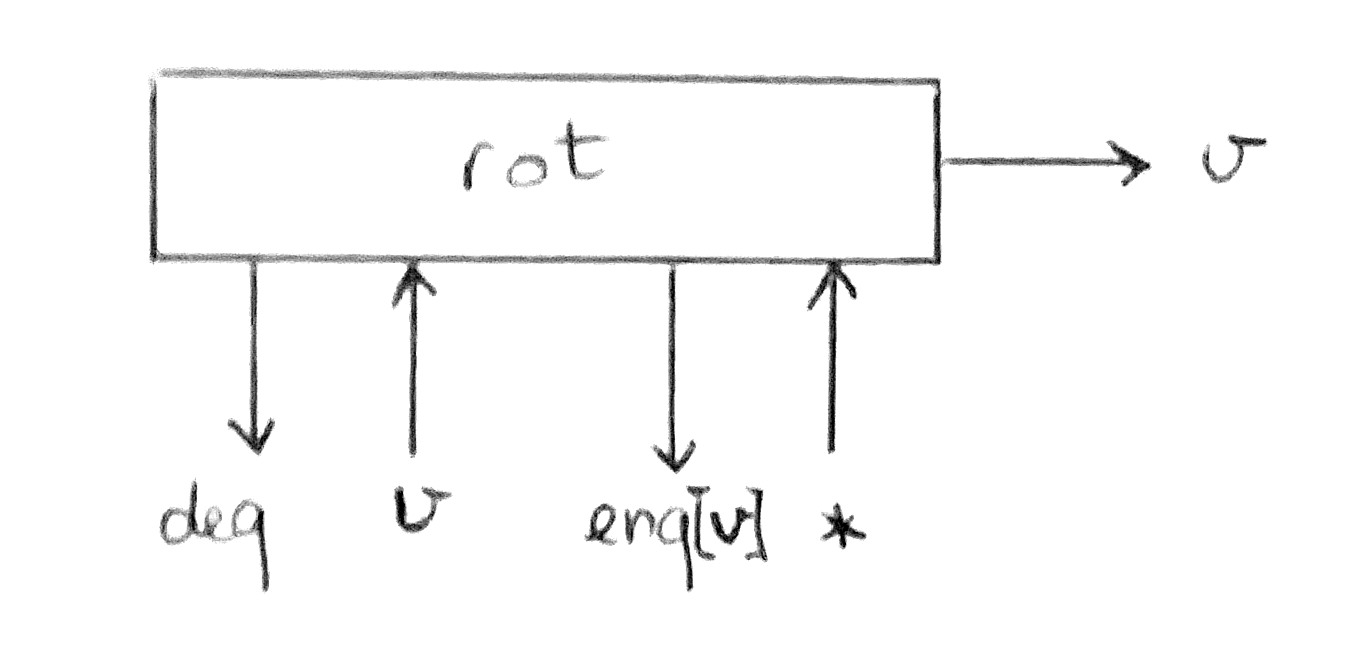
\includegraphics[scale=0.1]{rot}
\]
\end{frame}
%}}}

\begin{frame}{Plays}
More generally,
for a signature $E$ our game model
will use plays of the following form:
\[
  s \in \bar{P}_E(A) ::=
    \underline{v} \mid
    \underline{m} \mid
    \underline{m} n s
  \qquad
  (v \in A, m \in E, n \in \kw{ar}(m))
\]

This corresponds to behaviors of the following shape:
\[
  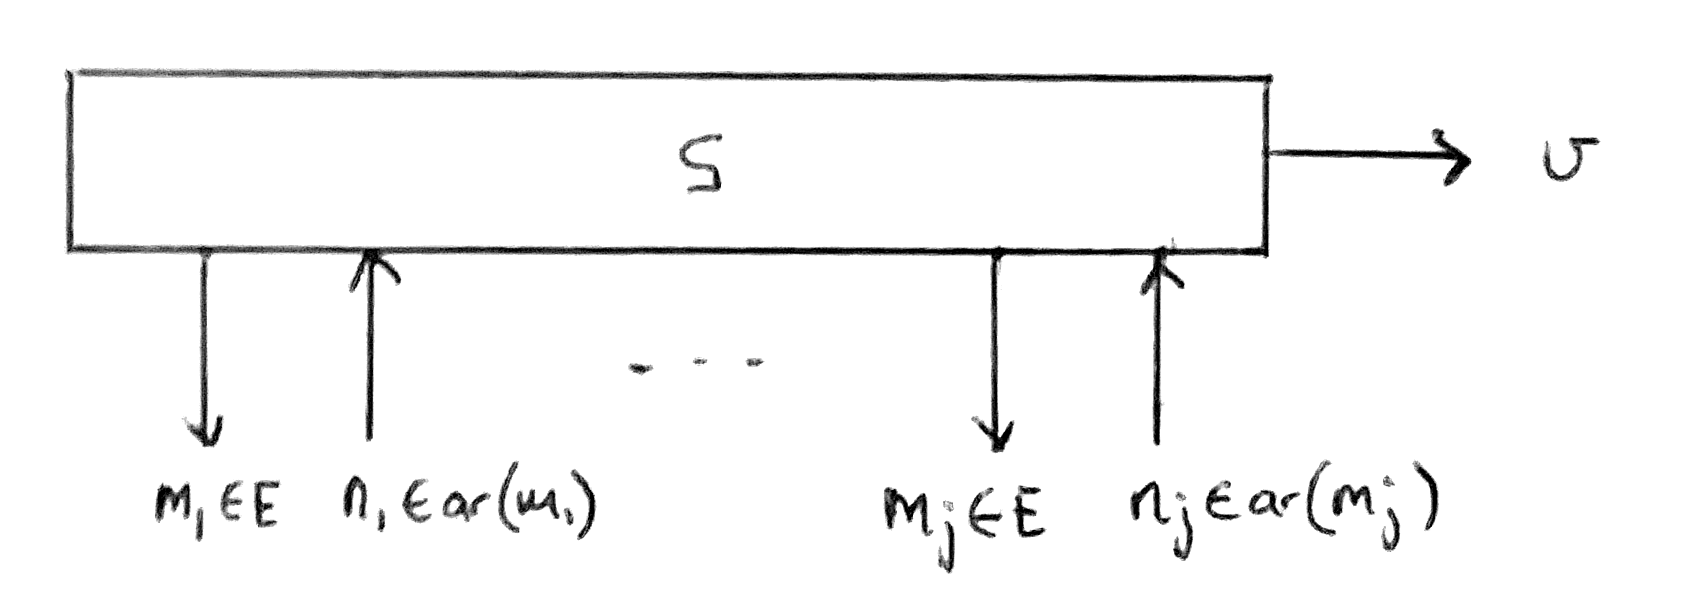
\includegraphics[scale=0.1]{play}
\]
\end{frame}

\begin{frame}{Strategies}
To define a category of strategies,
we to represent $f : E \rightarrow F$
which \emph{uses} outgoing calls in $E$
to \emph{implement} incoming calls in $F$.

We will use \emph{families} of the form
$(f^q)_{q \in F}$, where
$f^q \in \mathcal{I}_E(\kw{ar}(q))$.
This can be depicted as:
\[
  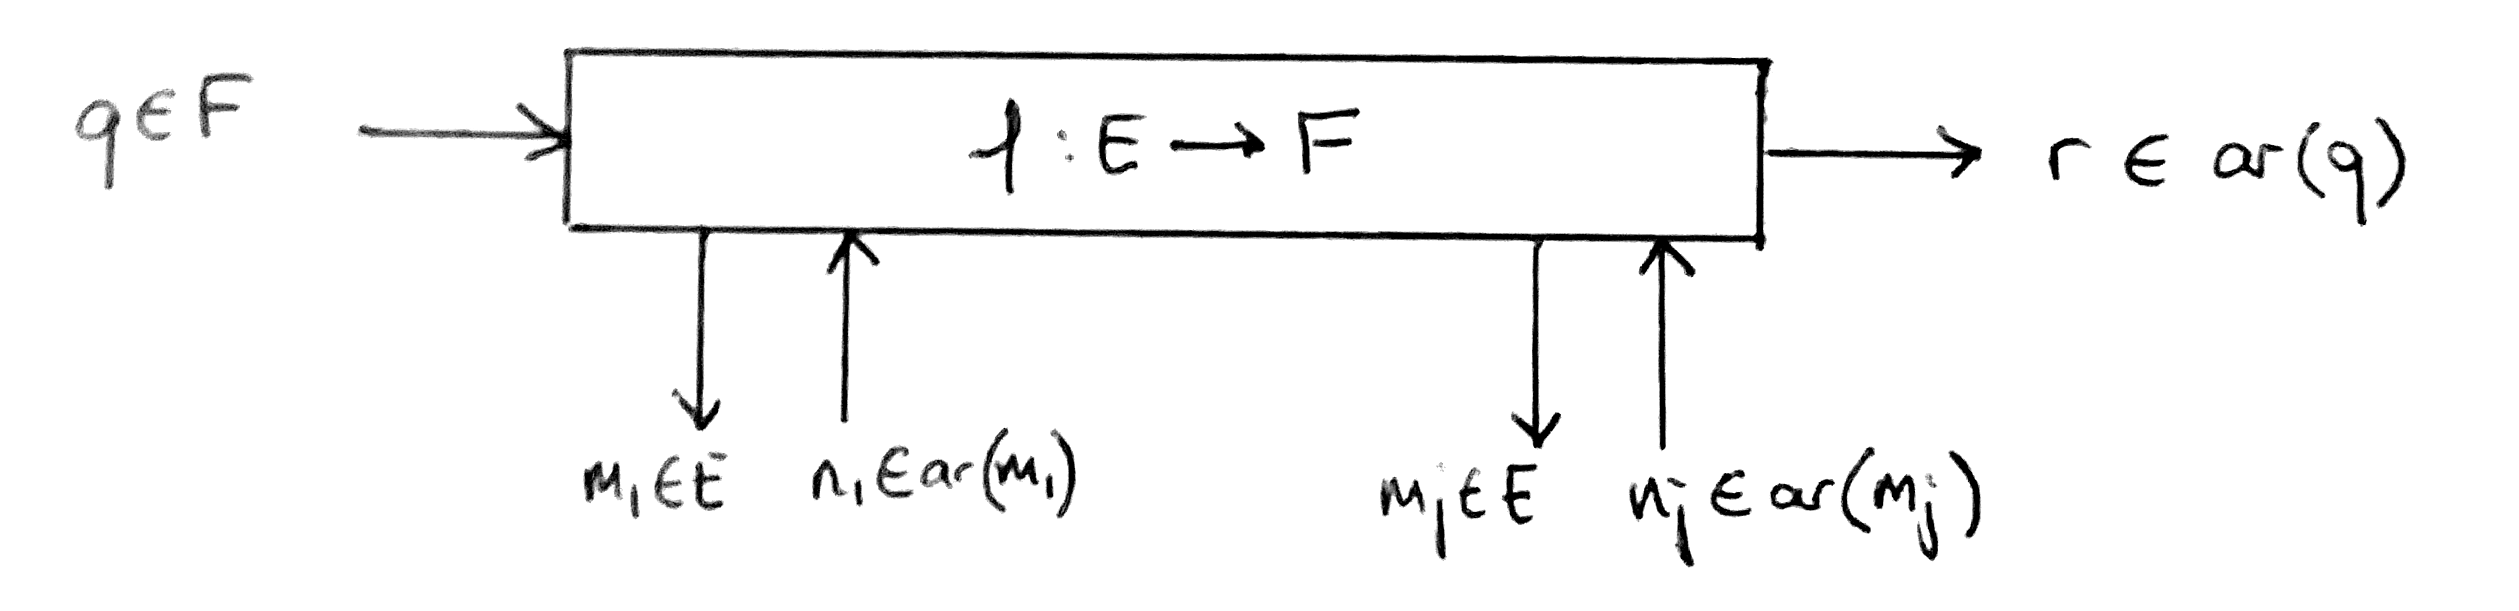
\includegraphics[scale=0.1]{mor}
\]
\end{frame}

\begin{frame}{Composition}
To compose $f : E \rightarrow F$ and $g : F \rightarrow G$,
we will substitute the $F$ calls in $g$ by
the correponding behavior given by $f$:
\[
  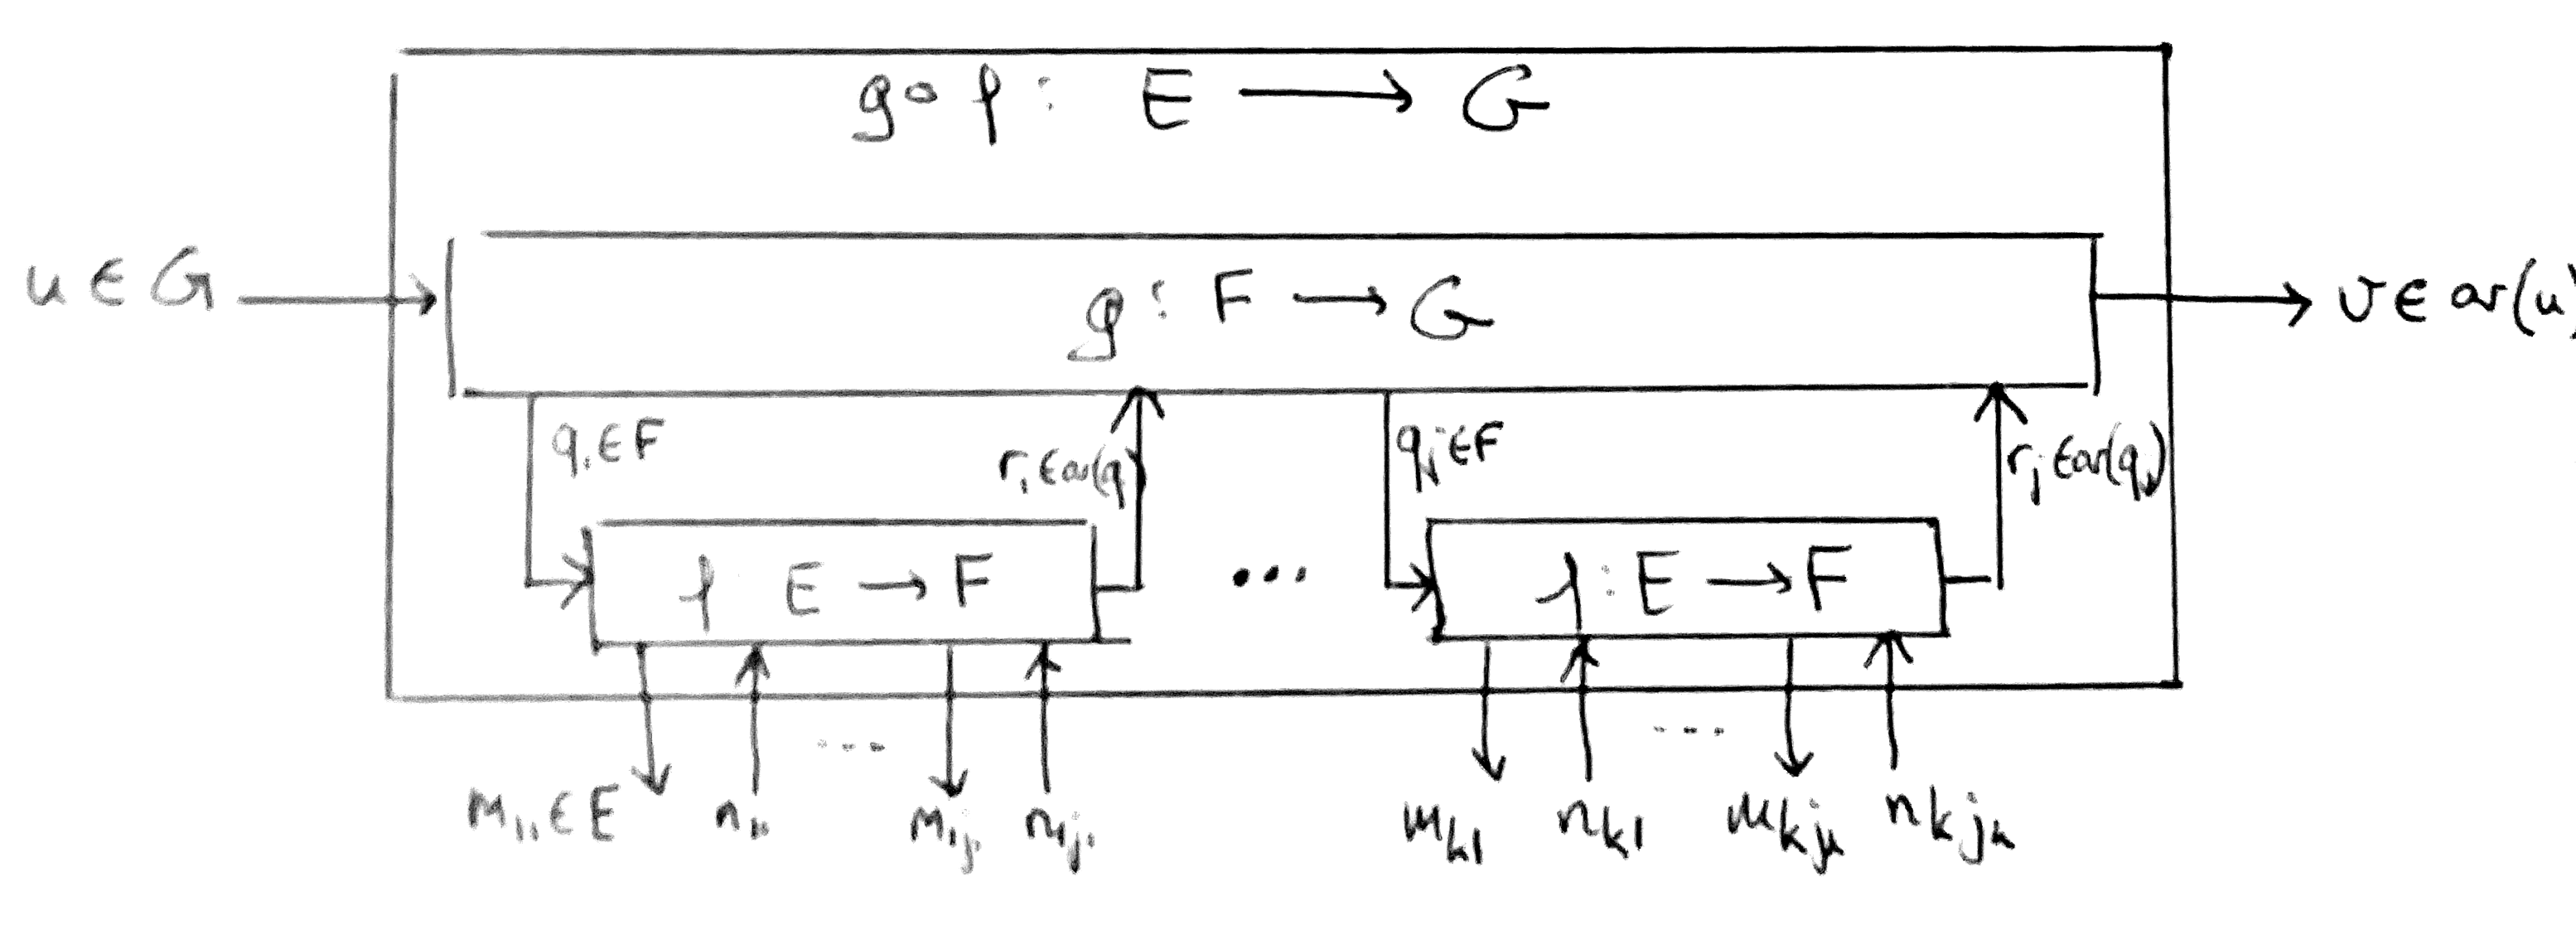
\includegraphics[scale=0.1]{comp}
\]
\end{frame}

\begin{frame}{Layers}
Given a set of abstract states $S$,
we can extend an effect signature $E$
to annotate all calls and returns with a state $k \in S$:
\[
  E@S :=
    \{ m@k : \kw{ar}(m) \times S \mid
       m \in E, k \in S \}
\]
These ingredients allow us to represent:
\begin{itemize}
  \item Layer interfaces as $L : 1 \rightarrow E@S$
  \item Layer implementations as $M : E_1 \rightarrow E_2$
  \item This can be promoted to $M@S : E_1@S \rightarrow E_2@S$
  \item Then $\llbracket M \rrbracket_L := M@S \circ L : 1 \rightarrow E_2@S$
\end{itemize}
\end{frame}

\begin{frame}{Abstraction}
To formulate correctness properties,
we will encode simulation relations as morphisms:
\[
  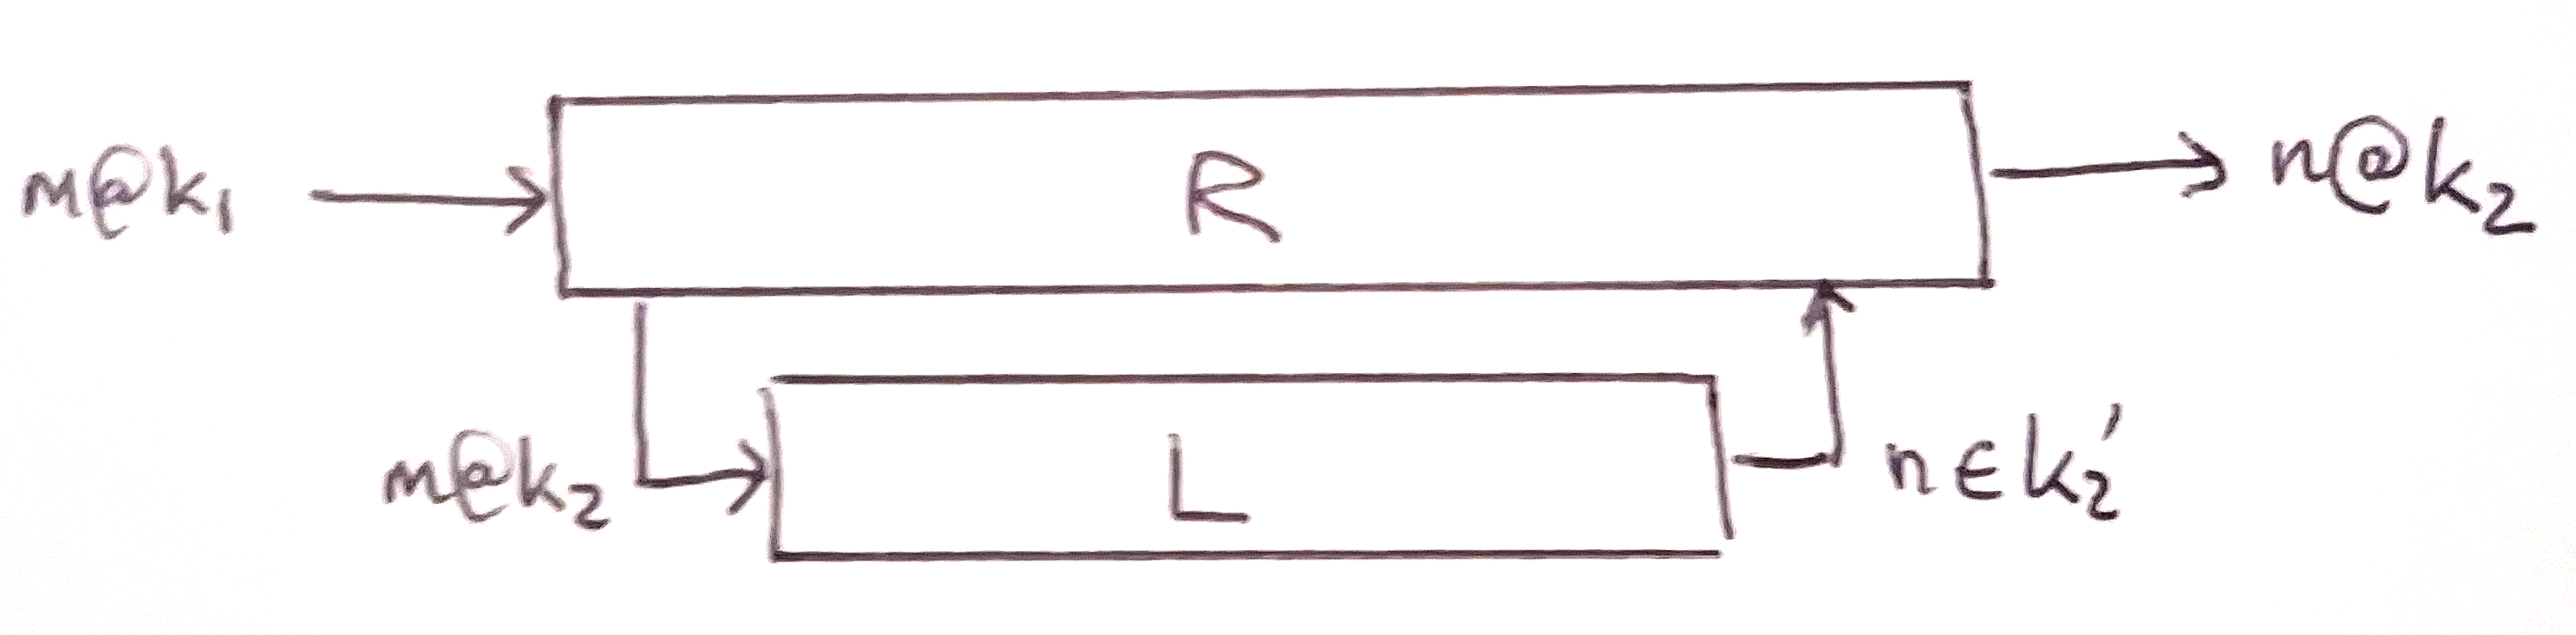
\includegraphics[scale=0.07]{simrel}
\]
and need to define an appropriate notion of refinement,
so that layer correctness can be expressed as:
\[
  R^*_{E_2} \!\circ L_2 \: \sqsubseteq \: \llbracket M \rrbracket_{L_1}
  \: \Leftrightarrow \:
  L_1 \vdash_R M : L_2
  \: \Leftrightarrow \:
  L_2 \: \sqsubseteq \: R_*^{E_2} \!\circ \llbracket M \rrbracket_{L_1} \,.
\]
However,
this requires a satisfactory treatment
of \emph{dual nondeterminism} and
\emph{alternating refinement}
in the context of our game model.
\end{frame}

%}}}

\section{Dual nondeterminism and refinement} %{{{

\begin{frame}{Refinement} %{{{
%\emph{Stepwise refinement} techniques
%treat programs, specifications and correctness
%in a uniform way.
%Specification constructs are added to the language,
%and the implementation is derived by
%incrementally replacing them
%by executable statements.

In the context of Hoare logic and axiomatic semantics,
a~refinement $C_1 \sqsubseteq C_2$
means that any correctness property satisfied by $C_1$
will also be satisfied by $C_2$:
\[
    C_1 \sqsubseteq C_2 \: := \:
    \forall P Q \bdot
      \htr{P}{C_1}{Q} \Rightarrow
      \htr{P}{C_2}{Q}
\]
%Then the goal is to establish
%a sequence of refinements
%$C_1 \sqsubseteq \cdots \sqsubseteq C_n$
%to show that a program $C_n$ involving
%only executable constructions
%correctly implements a specification $C_1$.

For games and open systems,
refinement is \emph{alternating}.
A refinement allows:
\begin{itemize}
  \item \emph{more} behaviors from the \emph{environment}
  \item \emph{fewer} behaviors form the system
\end{itemize}
\end{frame}
%}}}

\begin{frame}[fragile]{Angelic and demonic choice} %{{{
The \emph{refinement calculus} 
is a framework for stepwise refinement
of imperative programs,
constructed around predicate transformer semantics,
featuring \emph{dual nondeterminism}:
\begin{itemize}
  \item \emph{Angelic choices} are resolved by an angel:
  \[
    \begin{prooftree}
      \hypo{\htr{P}{C_1}{Q}}
      \infer1{\htr{P}{C_1 \sqcup C_2}{Q}}
    \end{prooftree}
    \qquad
    \begin{prooftree}
      \hypo{\htr{P}{C_2}{Q}}
      \infer1{\htr{P}{C_1 \sqcup C_2}{Q}}
    \end{prooftree}
  \]
  \item \emph{Demonic choices} are resolved by a demon:
  \[
    \begin{prooftree}
      \hypo{\htr{P}{C_1}{Q}}
      \hypo{\htr{P}{C_2}{Q}}
      \infer2{\htr{P}{C_1 \sqcap C_2}{Q}}
    \end{prooftree}
  \]
\end{itemize}
Angelic and demonic choices correspond to meets and joins
with respect to the refinement ordering.
%Two fundamental operations
%to make it possible to express specifications.
%
%By giving lattice structure,
%we obtain a model insensivive to branching.
%Complete distributivity further allows
%angelic and demonic choices to commute:
\end{frame}
%}}}

\begin{frame}{Completely distributive complete lattices} %{{{
The refinement calculus features \emph{unbounded}
angelic and demonic choices,
which work together as a
\emph{completely distributive lattice}:
\begin{itemize}
  \item Complete lattice: the model is insensitive to branching
  \item Complete distributivity: angelic and demonic choices commute
  \[
      \bigsqcap_{i \in I} \bigsqcup_{j \in J_i} x_{i,j} =
      \bigsqcup_{f \in (\prod_i J_i)} \bigsqcap_{i \in I} x_{i, f_i}
  \]
  \item $\bot$ is used to capture undesirable behaviors (only refines itself),
    including silent divergence.
\end{itemize}
Constructions are expected to be monotonic,
enabling congruent refinement.
Most preserve $\sqcup$ and $\sqcap$.
\end{frame}
%}}}

\begin{frame}{Strategies} %{{{
The traditional construction of strategies
uses \emph{angelic} nondeteminism
to range over the possible behaviors of the environment:
\[
  \mathcal{I}_E(A) := \mathcal{D}(\bar{P}_E(A))
\]
To enable demonic nondeterminism as well,
we will use the
\emph{free completely distributive lattice}
instead of downsets:
\[
  \mathcal{I}_E(A) := \mathbf{FCD}(\bar{P}_E(A))
\]
\end{frame}
%}}}

\begin{frame}[fragile]{Free completely distributive completion} %{{{
Morris and Tyrrell extended the refinement calculus
to functional programming by using
the \emph{free completely distributive lattice}
over a poset to capture dual nondeterminism as an effect:
\[
  \mathbf{FCD} : \mathbf{Pos} \rightleftarrows \mathbf{CDLat} : U
  \qquad
  \begin{tikzcd}
    C \arrow[r, "\phi"] \arrow[rd, "f"'] &
    \mathbf{FCD}(C) \arrow[d, "f^*_\phi", dashed] \\ & M
  \end{tikzcd}
\]
Each element $x \in \mathbf{FCD}(C)$ can be written as:
\[
  x = \bigsqcap_{i \in I} \bigsqcup_{j \in J_i} \phi(c_{ij})
  \qquad
  f^*_\phi(x) = \bigsqcap_{i \in I} \bigsqcup_{j \in J_i} f(c_{ij})
\]
In other words,
a complete homomorphism from $\mathbf{FCD}(C)$ into another lattice
is completely determined by its image on $C$.
\end{frame}
%}}}

\begin{frame}{Example: interaction primitives} %{{{
For $m : N \in E$,
we can use angelic nondeterminism to define
the interaction primitive $\mathbf{I}_E^m \in \mathcal{I}_E(N)$
as:
\[
  \mathbf{I}^m := \bigsqcup_{n \in N} \underline{m} n \underline{n}
\]
The family $\mathbf{I}_E : E \rightarrow E$
also serves as the identity morphism,
and can be depicted as:
\[
  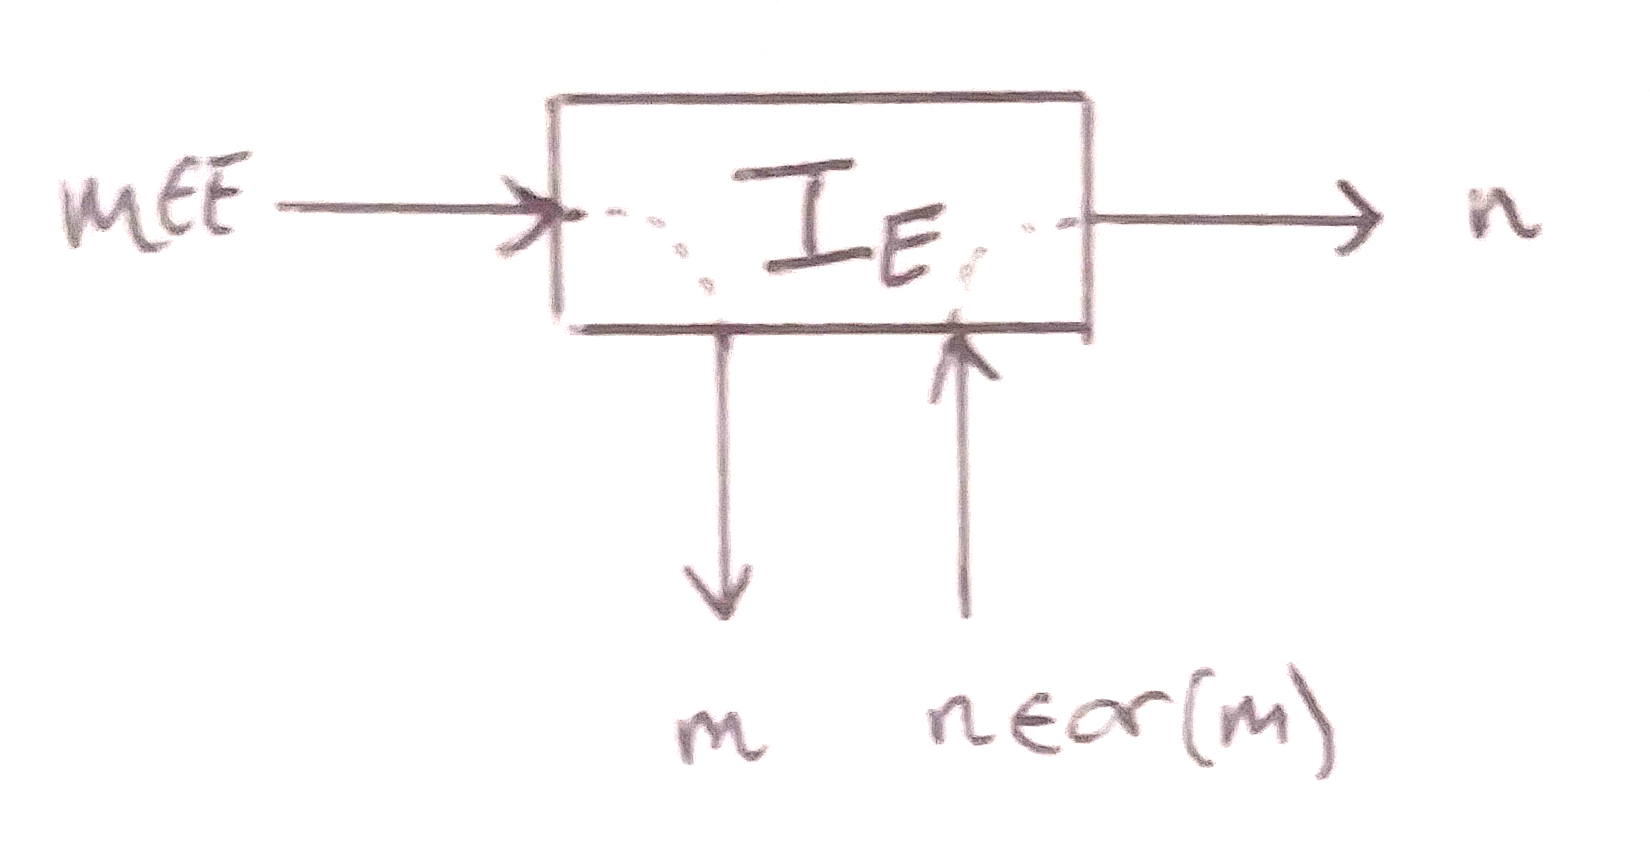
\includegraphics[scale=0.08]{int}
\]
\end{frame}
%}}}

\begin{frame}{Example: simulation relations} %{{{
We use dual nondeterminism,
to embed simulation relations as:
\[
  {\everymath={\displaystyle}
  \begin{array}{r@{\:}c@{\:}c@{\:}c@{\:}l}
  (R^*_E)^{m@k_1} := &
    \bigsqcup_{k_2 \in R^{-1}(k_1)} &
    n@k_2' \leftarrow \mathbf{I}^{m@k_2} ; &
    \bigsqcap_{k_1' \in R(k_2')} &
    \eta(n@k_1') \\[2.5em]
  (R_*^E)^{m@k_2} := &
    \bigsqcap_{k_1 \in R(k_2)} &
    n@k_1' \leftarrow \mathbf{I}^{m@k_1} ; &
    \bigsqcup_{k_2' \in R^{-1}(k_1')} &
    \eta(n@k_2')
  \end{array}}
\]
This establishes a Galois connexion
which we can use to model abstraction.
For $\sigma : 1 \rightarrow E@S_2$
and $\tau : 1 \rightarrow E@S_1$,
\[
  R^*_{E_2} \!\circ \sigma \: \sqsubseteq \: \tau
  \quad \Leftrightarrow \quad
  \sigma \: \sqsubseteq \: R_*^{E_2} \!\circ \tau \,.
\]
\end{frame}
%}}}

%}}}

\section{Conclusion} %{{{

\begin{frame}{Conclusion}
\end{frame}

%}}}

%\begin{frame}{Game semantics} %{{{
%Game semantics is an approach to compositional semantics:
%\begin{itemize}
%  \item Types are interpreted as \emph{games}
%    and terms as \emph{strategies}.
%  \item Very general, lots of research to build on.
%  \item Sometimes fairly complex.
%\end{itemize}
%
%For our purposes:
%\begin{itemize}
%  \item Type structure helps us model heterogenous systems;
%  \item First-order is good enough for system components,
%    this simplifies things a lot;
%  \item What about proofs?
%\end{itemize}
%\end{frame}
%%}}}

%\section{Effectful computations}
%
%\begin{frame}{Algebraic effects} %{{{
%In the framework of \emph{algebraic effects}:
%\begin{itemize}
%  \item Terms represent computations;
%  \item Operations represent effects;
%  \item Arguments specify possible continuations.
%\end{itemize}
%
%\begin{example}
%The term
%$\kw{readbit}(
%  \kw{print}["\text{Hello}"](\kw{done}),
%  \kw{print}["\text{World}"](\kw{done}))$
%can~be read as a strategy:
%\[
%  \begin{tikzpicture}[scale=0.8]
%    %\node (W) at (0,0) {};
%    \node (R) at (0,-1) {$\kw{readbit}$};
%    \node (W0) at (-2,-2) {$\kw{print}["\text{Hello}"]$};
%    \node (W1) at (+2,-2) {$\kw{print}["\text{World}"]$};
%    \node (K0) at (-2,-3) {$\kw{done}$};
%    \node (K1) at (+2,-3) {$\kw{done}$};
%    %\path (W) edge node[auto,swap] {$*$} (R);
%    \path (R) edge node[auto,swap] {0} (W0);
%    \path (R) edge node[auto] {1} (W1);
%    \path (W0) edge node[auto,swap] {$*$} (K0);
%    \path (W1) edge node[auto,swap] {$*$} (K1);
%  \end{tikzpicture}
%\]
%\end{example}
%\end{frame}
%%}}}
%
%\begin{frame}{Plays}
%\begin{definition}[Effect signature]
%A set $E$ of operations
%together with a mapping $\kw{ar} : E \rightarrow \mathbf{Set}$.
%\end{definition}
%
%\begin{example}
%\[
%  E_\kw{io} :=
%  \{ \kw{readbit} : \mathbbm{2}, \:
%     \kw{print}[s] : \mathbbm{1}, \:
%     \kw{done} : \varnothing \mid
%     s \in \kw{string} \}
%\]
%\end{example}
%
%\begin{definition}[Plays for interactions]
%The set $\bar{P}_E(A)$ is defined inductively by:
%\[
%  s \in \bar{P}_E(A) ::=
%    \underline{v} \mid
%    \underline{m} \mid
%    \underline{m} n s
%  \qquad
%  (v \in A, m \in E, n \in \kw{ar}(m))
%  \,,
%\]
%and ordered under prefix ($\underline{m} \sqsubseteq \underline{m} n s$).
%\end{definition}
%\end{frame}
%
%\begin{frame}[fragile]{Plays (drawing)}
%  \[
%  \begin{tikzpicture}[scale=0.5]
%    \draw[->] (0,1) -| (1,0) node[below left] {$m_1$} -- (1,-2);
%    \draw[->] (2,-2) -- (2,0) node[below right] {$n_1$};
%    \draw[->] (2,0) -- (2,1) -| (6,0) node[below left] {$m_2$} -- (6,-2);
%    {
%    \tikzset{xshift=5cm}
%    \draw[->] (2,-2) -- (2,0) node[below right] {$n_2$};
%    \draw[->] (2,0) -- (2,1) -| (6,0) node[below left] {$m_3$} -- (6,-2);
%    }
%    \tikzset{xshift=5cm}
%    \draw[->] (2,-2) -- (2,0) node[below right] {$n_1$};
%
%    \pmove{m_1} -- 
%
%  \end{tikzpicture}
%  \]
%\end{frame}

%
%
%\begin{frame}{Interaction specifications}
%The free completely distributive completion of
%$\bar{P}_E$
%gives us a version of the \emph{free monad}
%on the effect signature $E$.
%
%\begin{definition}[Interaction specification monad]
%\begin{itemize}
%  \item $\mathcal{I}_E(A) := \mathbf{FCD}(\bar{P}_E(A))$.
%  \item The unit $\eta^E_A : A \rightarrow \mathcal{I}_E(A)$
%    is defined by $\eta^E_A(v) := \underline{v}$
%  \item The extension of $f : A \rightarrow \mathcal{I}_E(B)$
%    is defined by:
%  \begin{align*}
%    f^\dagger(\underline{v}) &:= f(v) \\
%    f^\dagger(\underline{m}) &:= \underline{m} \\
%    f^\dagger(\underline{m} n s) &:=
%      \underline{m} \sqcup \underline{m} n f^\dagger(s)
%  \end{align*}
%\end{itemize}
%\end{definition}
%\end{frame}
%
%\begin{frame}{Summary}
%An \emph{interaction specification} in $\mathcal{I}_E(A)$
%triggers effects in $E$ and produces an outcome in $A$.
%
%$\mathcal{I}_E(A)$ is equipped with a completely distributive lattice
%structure which models \emph{dual nondeterminism}.
%\end{frame}
%
%\section{Strategies}
%
%\begin{frame}{Interaction primitives and substitution}
%A strategy specification $f : E \rightarrow F$
%is a \emph{family} $(f^m)_{m \in F}$:
%\[
%     f^m \in \mathcal{I}_E(\kw{ar}(m)) \qquad
%     (m \in F)
%\]
%The identity strategy $\mathbf{I} : E \rightarrow E$
%is the family of \emph{interaction primitives}:
%\[
%  \mathbf{I}_E^m :=
%    \bigsqcup_{n \in \kw{ar}(m)} \underline{m} n \underline{n}
%\]
%The composition of $f : E \rightarrow F$ and $g : F \rightarrow G$
%will be defined as:
%\[
%    (g \circ f)^m := g^m[f]
%\]
%\end{frame}
%
%\begin{frame}{Interaction substitution}
%Given $x \in \mathcal{I}_F(A)$ and $f : E \rightarrow F$,
%the \emph{interaction substitution} $x[f] \in \mathcal{I}_E(A)$
%is defined by:
%\begin{align*}
%  \underline{v}[f] &:= \underline{v} \\
%  \underline{m}[f] &:= r \leftarrow f^m ; \bot \\
%  \underline{m}ns[f] &:= r \leftarrow f^m ; \{r = n\} ; s[f] \,.
%\end{align*}
%\end{frame}

\end{document}
